\documentclass{article}

\usepackage{microtype}
\usepackage{graphicx}
\usepackage{booktabs}
\usepackage{multirow}
\usepackage{xcolor}
\usepackage{hyperref}
\usepackage[preprint]{icml2026}
\usepackage[capitalize,noabbrev]{cleveref}

% Red marker for numbers still to be filled in from the final Analysis 2 run; none should remain at submission.
\newcommand{\tbd}[1]{\textcolor{red}{#1}}

\makeatletter
\renewcommand{\ICML@preprint}{\textit{11-777 Second Project Assignment, Fall 2026.}}
\makeatother

\icmltitlerunning{11-777 Second Project Assignment}

\begin{document}

\twocolumn[
  \icmltitle{\texorpdfstring{11-777 Second Project Assignment\\[0.25em]
  \large Team 7: Efficient Multimodal Reasoning}
  {11-777 Second Project Assignment: 7: Efficient Multimodal Reasoning}}

  \begin{icmlauthorlist}
    \icmlauthor{Nikkita Batra (nbatra)}{cmu}
    \icmlauthor{Arjun Shah (aashah2)}{cmu}
    \icmlauthor{Alvin Wang (alvinw2)}{cmu}
    \icmlauthor{Lindy Zhang (lindyz)}{cmu}
  \end{icmlauthorlist}

  \icmlaffiliation{cmu}{Carnegie Mellon University, Pittsburgh, Pennsylvania, USA}
\icmlcorrespondingauthor{Nikkita Batra}{nbatra@andrew.cmu.edu}

  \icmlkeywords{multimodal machine learning, dataset analysis, modality analysis}
  \vskip 0.3in
]

\printAffiliationsAndNotice{}

\section{Project Repository}

\href{https://github.com/alvinwang1/multimodal-reasoning-project/}
{github.com/alvinwang1/multimodal-reasoning-project}. Each analysis has its own folder
(\texttt{src/analysis\_\{a,b,c\}}) and a README section; all figures are regenerated from the logged outputs.

\section{Introduction}

Our project asks how a multimodal model should allocate computation across
image, audio, and text inputs while preserving reasoning accuracy. We study
this on OmniBench \citep{li2025omnibench}, whose 1,142 multiple-choice
questions each pair an image, an audio clip (speech, sound event, or music),
and a text question, together with a generated image caption and an audio
transcript.

Each of the research ideas in our proposal rests on an assumption about the
data that we had not yet verified. Adaptive representation routing (Idea~1)
assumes that the cheapest sufficient representation differs across examples,
and that this can be predicted from inexpensive signals such as the question
text. The marginal-utility study (Idea~3) assumes that image and audio
contribute unequally and that this imbalance varies by task and audio type.
Replacing raw inputs with text surrogates (Idea~4) assumes that captions and
transcripts are much cheaper than the raw modalities while preserving the
information needed to answer.

We test these assumptions with three analyses on a fixed, seeded subset of 90
OmniBench items (30 per audio type). \Cref{sec:a1} is a human simulation in
which team members first see only the question, caption, and transcript, judge
whether this text suffices, and then reveal the raw image and audio before
answering. \Cref{sec:a2} is a data analysis that uses Qwen2.5-Omni-3B
\citep{xu2025qwen25omni} as a probe to measure the accuracy and token cost of
seven raw and surrogate input configurations, and uncovers a strong
answer-position bias in the benchmark. \Cref{sec:a3} explores the language
modality, testing whether sentence embeddings and interpretable lexical
features carry enough signal to decide when text alone suffices.
\Cref{sec:discussion} uses these results to revise our research ideas.

% ---------------------------------------------------------------------------
\section{Analysis 1: Can People Tell When Text Is Enough?}
\label{sec:a1}

\paragraph{Setup.} Each of the four authors annotated 20 items (10 shared by
all, 10 unique; 50 distinct items, balanced by audio type) in a staged-reveal
tool. Stage~0 shows the question, the four options, the image caption, and the
audio transcript. The annotator records whether this text is enough to answer
(yes/no), a confidence (1--5), and an optional answer. They then choose
\emph{reveal image}, \emph{reveal audio}, or \emph{answer now}; every step is
logged in order. The final answer comes with a confidence and a free-text note
on which input decided it. Gold answers were never shown.

\paragraph{Hypotheses.} (H1.1) Annotators can tell when text suffices: their
text-only answers should be more accurate when they say ``yes''. (H1.2) Revealing
the raw modalities improves accuracy, most for sound events, whose transcripts
are only short descriptions. (H1.3) Annotators agree with each other, and with
the model, about which items are text-sufficient.

\begin{table}[t]
\caption{Staged-reveal results per annotator (20 items each). \emph{Text}: accuracy of the optional stage-0
answer; \emph{Final}: after revealing; \emph{W$\to$R/R$\to$W}: answers changed from wrong to right and
right to wrong after revealing; \emph{Said enough}: share of ``text is enough'' judgments; \emph{Judg.}:
how often that judgment matched whether the annotator's text-only answer was correct.}
\label{tab:annotators}
\centering\small
\setlength{\tabcolsep}{3.5pt}
\begin{tabular}{lcccccc}
\toprule
 & Text & Final & W$\to$R & R$\to$W & Said enough & Judg. \\
\midrule
A1 & 60 & 40 & 1 & 5 & 60 & 60 \\
A2 & 28 & 55 & 6 & 0 & 40 & 78 \\
A3 & 37 & 50 & 3 & 1 & 70 & 42 \\
A4 & 26 & 35 & 3 & 2 & 80 & 42 \\
\midrule
All & 38 & 45 & 13 & 8 & 63 & 55 \\
\bottomrule
\end{tabular}
\end{table}

\paragraph{Results.} \Cref{tab:annotators} summarizes the annotations.
Text-only answers were 38.2\% accurate ($n{=}76$); after revealing, accuracy
rose to 45.0\%, with 13 answers fixed and 8 broken. The ``text is enough''
judgment was weakly informative: text-only accuracy was 45\% when annotators said
yes versus 26\% when they said no, but the judgment matched actual text-only
correctness only 55\% of the time, and annotators said yes on 63\% of items. In
79 of 80 items annotators revealed \emph{both} modalities, almost always image
first (78/80), even when they had judged the text sufficient. Agreement on the
10 shared items was low: Fleiss' $\kappa{=}0.08$ for the sufficiency judgment and
$0.22$ for the final answer; all four agreed on only one item, nobody answered
three items correctly, and a majority vote was only 40\% accurate. Human
sufficiency judgments were unrelated to the model's text-sufficient labels
(\cref{sec:a2}): Cohen's $\kappa{=}0.00$ on the 50 items, with humans saying yes
far more often (66\% vs.\ 18\%). In the free-text notes, audio was cited as
decisive in 33 cases, the image in 31, and text in 26 (notes can cite several).

\paragraph{Discussion.} H1.1 holds only weakly: people are overconfident that
text suffices, and individual annotators differ widely (one was 60\% accurate
from text alone and lost five correct answers after revealing, another gained
six). H1.2 is supported on average, but extra modalities help less than
expected and can hurt. H1.3 is rejected: sufficiency is not a stable property
that people agree on. Two caveats limit these conclusions. First, revealing was
free, so annotators had no incentive to stop early; the reveal \emph{order}
(image first) is informative, but stopping behavior is not, and a cost per reveal
is needed to simulate a router. Second, final human accuracy (45\%) equals the
always-``D'' baseline on these items (\cref{sec:a2}), and agreement is low,
which suggests that a substantial share of OmniBench items are ambiguous. This
caps the accuracy differences any efficiency method can show on the benchmark.

% ---------------------------------------------------------------------------
\section{Analysis 2: Raw Modalities vs.\ Text Surrogates}
\label{sec:a2}

\paragraph{Setup.} We run Qwen2.5-Omni-3B (text output only, bf16, Apple M2 Max)
on the 90-item subset under seven input configurations; the question and options
are always present, and captions or transcripts are inserted as text in place of
the raw modality: image+audio (full), image+transcript, caption+audio,
caption+transcript, image only, audio only, and question only. Each item is
scored with one forward pass by a softmax over the next-token logits of the
letters A--D (single tokens; greedy generation agreed with the argmax letter on
all 55 checked passes). Images are capped at 768 visual tokens (mean 700); audio
costs 25 tokens/s. Every configuration is run under three option orders (the
original and two seeded shuffles), and we report accuracy averaged over orders.
We log input tokens by modality, forward latency (batch size 1, warm-up, device
synchronization), and activation memory.

\paragraph{Hypotheses.} (H2.1) Text surrogates cut input cost by more than half
with little accuracy loss. (H2.2) Raw audio matters for sound events but can be
replaced by a transcript for speech. (H2.3) The cheapest sufficient configuration
varies across items, leaving headroom for routing.

\begin{figure}[t]
\centering
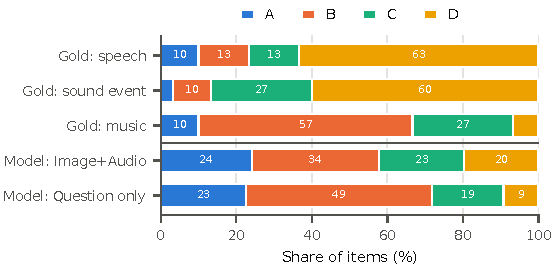
\includegraphics[width=\columnwidth]{figures/position_bias.pdf}
\caption{Position of the correct answer in our subset (top three rows) vs.\ the letter the model predicts
(bottom two rows, all option orders). Across all 1,141 OmniBench items the answer is ``D'' 49\% of the time
(``A'': 9\%); music is the exception. The model favors ``B'' regardless of input.}
\label{fig:position}
\end{figure}

\paragraph{Answer position is a confound.} OmniBench's correct answers are
heavily skewed toward ``D'' (49\% of all items; 63\% of speech and 60\% of
sound-event items in our subset), except for music, where ``B'' dominates
(57\%; \cref{fig:position}). The model independently prefers ``B'' (34--49\% of its
predictions in every configuration, including question only). These two biases
interact: in the original order, music looks easy and speech looks hard. A
trivial always-``D'' baseline scores 43\% on our subset, above the model's
original-order accuracy with full input (38.9\%). Averaging over option orders
removes most of this effect, so all accuracies below are order-averaged.

\begin{table}[t]
\caption{Accuracy (\%, mean over three option orders; 30 items per audio type), mean input tokens, and mean
forward latency per configuration.}
\label{tab:configs}
\centering\small
\setlength{\tabcolsep}{3pt}
\begin{tabular}{lcccccc}
\toprule
Input & Speech & Sound & Music & All & Tokens & Lat. (s) \\
\midrule
Image+Audio        & 42.2 & 36.7 & 54.4 & 44.4 & 1105 & 3.3 \\
Image+Transcript   & \textbf{48.9} & 32.2 & \textbf{70.0} & \textbf{50.4} & 861 & 2.7 \\
Caption+Audio      & 31.1 & 40.0 & 43.3 & 38.1 & 671 & 1.4 \\
Caption+Transcript & 36.7 & \textbf{43.3} & 65.6 & 48.5 & 427 & 0.8 \\
Image only         & 31.1 & 16.7 & 60.0 & 35.9 & 834 & 2.6 \\
Audio only         & 34.4 & 42.2 & 53.3 & 43.3 & 403 & 1.0 \\
Question only      & 22.2 & 23.3 & 44.4 & 30.0 & 132 & 0.3 \\
\bottomrule
\end{tabular}
\end{table}

\begin{figure}[t]
\centering
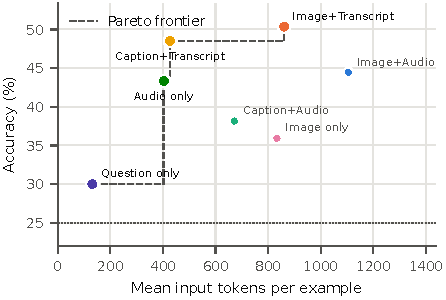
\includegraphics[width=\columnwidth]{figures/acc_vs_tokens.pdf}
\caption{Accuracy (mean over option orders) vs.\ mean input tokens; the dashed line is the Pareto frontier.}
\label{fig:pareto}
\end{figure}

\paragraph{Results.} \Cref{tab:configs,fig:pareto} summarize accuracy and cost.
Caption+transcript matches the full input (48.5\% vs.\ 44.4\%; paired difference
$+4.1$ points, bootstrap 95\% CI $[-4.8, 13.3]$) with 39\% of the tokens, a quarter
of the latency (0.8\,s vs.\ 3.3\,s), and 126\,MB vs.\ 327\,MB of activation memory.
Image+transcript is the most accurate configuration (50.4\%). Replacing raw audio by
its transcript helps: with the caption present, accuracy rises from 38.1\% to
48.5\% ($+10.4$, CI $[3.0, 17.8]$, Wilcoxon $p{=}0.007$). Replacing the image by
its caption costs a few points on average (50.4\% $\to$ 48.5\%), but the effect
depends on audio type: the raw image helps on speech items (48.9\% vs.\ 36.7\%,
$p{=}0.047$) and hurts on sound events (32.2\% vs.\ 43.3\%, n.s.). On sound
events, audio alone beats image alone by 25.6 points ($p{=}0.014$), consistent
with H2.2. Raw audio does carry information (audio only vs.\ question only:
$+13.3$, $p{=}0.002$), yet the model uses it worse than a short transcript.
Predictions are fragile: across the three orders, the model gives the same answer
on only 58--71\% of items for any configuration and 33\% for question only.

An oracle that picks, for each item, the cheapest configuration that is correct
under all three orders reaches 57.8\% at 25\% of the full-input cost; 38 of 90 items
are not robustly solved by any configuration, and caption+transcript is the
cheapest robust solution for 21 items. Requiring robustness matters: an oracle
over the original order alone reports 68.9\%, inflated by lucky guesses. A
confidence cascade that starts from caption+transcript and escalates to the full
input when the maximum option probability is below $\tau$ peaks at 50.7\% at 67\%
of the cost ($\tau{=}0.565$), barely above caption+transcript alone, because the
input it escalates to is not more accurate than its starting point. Under a
utility $U{=}\text{acc}-\lambda\cdot\text{cost}$, caption+transcript is optimal for
all $\lambda\in[0.05, 0.68]$.

\paragraph{Discussion.} H2.1 is supported: for this model, text surrogates are
much cheaper and at least as accurate as the raw inputs. H2.2 is supported in
direction (audio matters most for sound events, the image most for speech), but
the model exploits raw audio poorly overall. H2.3 is supported: the cheapest
sufficient configuration varies widely across items, and a permutation-robust
oracle still leaves 13 points of headroom at a quarter of the cost. Two
qualifications matter for Idea~4. The cost advantage depends on audio type, since
music captions and descriptions are long (caption+transcript reaches up to 72\% of
the full-input cost on music items). And for sound events and music the
``transcript'' is a human-written description of the audio rather than a
transcription, so it hands the model information that a raw-audio pipeline would
need to extract itself.

% ---------------------------------------------------------------------------
\section{Analysis 3: Language Modality}
\label{sec:a3}

\paragraph{Setup.} For each of the 90 items we build three text views: the
question, the question with caption and transcript, and the transcript alone.
We embed each with Sentence-BERT (\texttt{all-mpnet-base-v2};
\citealp{reimers2019sentencebert}) and compute 194 normalized Empath
categories \citep{fast2016empath}. We visualize the embeddings with t-SNE
\citep{vandermaaten2008tsne} and predict whether text is enough with four
predictors, using stratified 5-fold cross-validation and AUROC: (a) logistic
regression on embeddings, (b) logistic regression on Empath features, (c) the
model's maximum option probability under caption+transcript (no training), and
(d) the majority class. The \emph{model label} marks an item text-sufficient if
caption+transcript is correct under all three option orders (32/90, 36\%:
speech 20\%, sound 30\%, music 57\%). We repeat the predictions with the human
majority ``text is enough'' judgment from \cref{sec:a1} (50 items, 66\% yes).

\paragraph{Hypotheses.} (H3.1) The question text alone encodes whether an item
needs raw inputs, which would make a question-only router viable. (H3.2)
Interpretable lexical categories identify which content tends to be
text-answerable.

\begin{figure}[t]
\centering
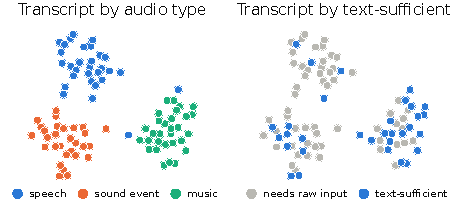
\includegraphics[width=\columnwidth]{figures/tsne_transcript_pair.pdf}
\caption{t-SNE of transcript embeddings. Transcripts separate cleanly by audio type (left), but
text-sufficient items do not cluster (right).}
\label{fig:tsne}
\end{figure}

\begin{table}[t]
\caption{AUROC (mean $\pm$ std over 5 folds) for predicting text-sufficiency. Model labels: $n{=}90$;
human labels: $n{=}50$. Q = question, QCT = question+caption+transcript, T = transcript.}
\label{tab:auroc}
\centering\small
\setlength{\tabcolsep}{4pt}
\begin{tabular}{llcc}
\toprule
Predictor & View & Model labels & Human labels \\
\midrule
\multirow{3}{*}{SBERT + LR}  & Q   & .54 $\pm$ .12 & .27 $\pm$ .09 \\
                             & QCT & .55 $\pm$ .07 & .26 $\pm$ .05 \\
                             & T   & .70 $\pm$ .13 & .46 $\pm$ .09 \\
\multirow{3}{*}{Empath + LR} & Q   & .58 $\pm$ .06 & .42 $\pm$ .18 \\
                             & QCT & .47 $\pm$ .06 & .55 $\pm$ .29 \\
                             & T   & .60 $\pm$ .07 & .57 $\pm$ .17 \\
Omni max prob                & --  & \textbf{.73 $\pm$ .11} & \textbf{.73 $\pm$ .15} \\
Majority class               & --  & .50 & .50 \\
\bottomrule
\end{tabular}
\end{table}

\paragraph{Results.} The embeddings capture coarse structure: question
embeddings group by task type (cosine silhouette 0.12) and transcript
embeddings separate almost perfectly by audio type (0.19; \cref{fig:tsne}), but
text-sufficient items do not cluster in any view ($|\text{silhouette}|\le0.02$).
\Cref{tab:auroc} shows that the question text alone barely predicts the model
label (AUROC 0.54), while transcript embeddings reach 0.70. The best predictor is
the model's own confidence under caption+transcript (0.73), which needs no
training and also predicts the \emph{human} judgment equally well (0.73).
Text-only predictors of the human label fall below 0.5; with 50 items this is the
expected behavior of cross-validation when features carry no signal, not
evidence of an inverse relationship. The transcript learning curve rises from
0.58 at 10\% of the training data to 0.70 at 70\% and then plateaus, with fold
standard deviations around 0.1. No Empath category is significantly associated
with the model label after Benjamini--Hochberg correction (strongest:
\emph{love}, $r{=}0.30$, uncorrected $p{=}0.004$, $q{=}0.35$).

\paragraph{Discussion.} H3.1 is rejected: the question text does not reveal
whether raw inputs are needed. Transcript embeddings do better largely because
they encode the audio type, which correlates with text-sufficiency (music items
are most often text-sufficient). H3.2 is not supported at this sample size. The
practical signal for routing is the model's confidence after a cheap
text-surrogate pass, which agrees with both model-derived and human sufficiency
labels.

% ---------------------------------------------------------------------------
\section{Discussion}
\label{sec:discussion}

\paragraph{Benchmark and evaluation.} Two properties of OmniBench change how we
will evaluate every idea. Correct answers are concentrated at position ``D''
(49\%), and the model prefers ``B'', so single-order accuracy is biased; an
always-``D'' baseline beats the full model. Humans reach only 45\% with all
inputs and agree weakly, which suggests many items are ambiguous. We will
therefore report accuracy averaged over option permutations, include
position-prior baselines, and treat accuracy differences of a few points on
small subsets as noise.

\paragraph{Idea 4 (text surrogates).} Our results support the premise more
strongly than expected: for Qwen2.5-Omni-3B, caption+transcript matches or beats
the full input at 39\% of the tokens and about a quarter of the latency. We will
(i) separate speech transcripts from non-speech audio \emph{descriptions},
which are not cheap transcriptions but human-written summaries; (ii) account for
long music captions, where the cost advantage shrinks; and (iii) compare against
model-generated captions and transcripts, since OmniBench's surrogates are not
available at deployment time and their cost must include generating them.

\paragraph{Idea 1 (adaptive routing).} The oracle shows large headroom, but our
analyses change how a router should work. The question text carries almost no
signal (AUROC 0.54), and human sufficiency judgments are unreliable targets
($\kappa{=}0.08$ between people, $0.00$ with the model). The model's confidence
after a caption+transcript pass is the best cheap signal (AUROC 0.73). We will
therefore redesign the router as a confidence-based cascade that starts from
text surrogates and escalates to the configuration that adds the most
information (image+transcript rather than the full input), and train its targets
on permutation-robust correctness, so that chance-level ``wins'' of cheap
configurations do not dominate the labels.

\paragraph{Idea 3 (marginal utility).} Image and audio contribute unequally, and
the imbalance flips with audio type: the raw image adds 12 points over its caption
on speech items, while on sound events audio alone beats image alone by 26 points.
Raw audio is worth less than its transcript for this model, and humans revealed
the image first in nearly all cases. Budget sweeps should therefore vary image and
audio tokens separately per audio type, and treat text surrogates as a third
option competing for the same budget.

\paragraph{Idea 2 (audio adaptation).} We did not test this idea directly, but
the gap between raw audio and its transcript motivates it: adaptation should be
measured against a transcript baseline, not only against a model without audio.

\bibliography{references}
\bibliographystyle{icml2026}

\clearpage
\appendix

\section{AI/LLM Usage Disclosure}

\textbf{[Team: review and complete this section; it must describe all AI use accurately.]}

We used Claude Code (Anthropic, model Claude Opus 5.5) as a coding and writing assistant. Specifically:
\begin{itemize}
  \item \textbf{Planning:} discussing the analysis plan, backend choice for running Qwen2.5-Omni-3B locally
    on Apple Silicon, and subset size.
  \item \textbf{Code:} writing most of the analysis code in the repository (data subset selection, the
    Analysis~2 model runner and analysis scripts, the Gradio annotation tool for Analysis~1 and its
    analysis script, and the Analysis~3 feature extraction, t-SNE, and prediction scripts), and running
    the scripts. The team reviewed the outputs, made the design decisions (analyses, subset size, number
    of option orders, annotation protocol), and launched the main model runs.
  \item \textbf{Analysis:} the assistant flagged the answer-position bias and suggested averaging over
    option orders; the team decided to adopt this.
  \item \textbf{Writing:} the assistant drafted parts of this report from the computed results; the team
    revised the text. \textbf{[Team: describe what you changed.]}
  \item \textbf{Annotation:} all human annotations in Analysis~1 were produced by the four authors; no AI
    model produced or edited annotation data.
\end{itemize}

\section{Teammate Contributions}

\textbf{[Team: fill in each person's contributions to idea development, coding and debugging, literature
review, annotation, and writing.]}

\begin{itemize}
  \item \textbf{Nikkita Batra:} annotation (Analysis~1); \textbf{[...]}
  \item \textbf{Arjun Shah:} annotation (Analysis~1); \textbf{[...]}
  \item \textbf{Alvin Wang:} annotation (Analysis~1); \textbf{[...]}
  \item \textbf{Lindy Zhang:} annotation (Analysis~1); \textbf{[...]}
\end{itemize}

\end{document}
